Puntos a abordar

- mencionar realizabilidad clásica. Related work capaz en la conclusión
- hacer una investigación de otras formas de hacer witness extraction. Capaz no es original lo nuestro (y capaz Coq lo banca con realizabilidad).

\begin{itemize}
    \item Motivación, limitaciones de lógica clásica. Demostración sqrt 2
    \item Lógica intuicionista
    \item Como necesitamos reducir en ND, necesitamos la demo en ND. Escribirla
          en este caso.
    \item También queremos para $\classPiTwo$, mostrar la extensión en ND.
    \item En realidad no nos sirve $\transDNeg{\Gamma}$, queremos dejarlo como
          está y demostrar que los axiomas demuestran sus traducciones. Pero no vale
          siempre (buscar c.ej), caracterizar cuando.
    \item Sumarizar cómo queda, vincular con reducción. Mostrar ejemplos en PPA
          que funcionan y ejemplos que no.
    \item Extensión a demostraciones. Mostrar algunos ejemplos interesantes (y
          los que usen los lemas dNegRElim y rElim)
    \item Lemas para demostraciones: dNegRElim (relacionar con \ref{ppa-cert:sec:abs-reasoning}), rElim, tNegRElim
    \item Reducción (buena explicación
          \url{https://plato.stanford.edu/entries/natural-deduction/}). En realidad se
          conoce como \textbf{normalization}.
          \begin{itemize}
              \item Similitud con reducción en cálculo lambda.
              \item Ejemplos de LP y todo LPO
              \item substHyp, substVar en proofs
              \item Argumentos de que es correcto y completo?
              \item Small step vs big step
          \end{itemize}
\end{itemize}

\newpage

En los capítulos anteriores vimos como el lenguaje PPA puede ser usado para
escribir demostraciones de alto nivel, que son certificadas generando
demostraciones de bajo nivel usando el sistema lógico de deducción natural.
Ahora vamos a introducir una nueva funcionalidad: la \textbf{extracción de testigos}.

\begin{multicols}{2}
    \begin{figure}[H]
        \lstinputlisting{listings/extract/exists.ppa}
        \caption{Extracción simple}
        \label{fri:prog:exists}
    \end{figure}

    \begin{figure}[H]
        \lstinputlisting{listings/extract/forall.ppa}
        \caption{Extracción con instanciación}
        \label{fri:prog:forall}
    \end{figure}
    \begin{figure}[H]
        \lstinputlisting[firstline=2]{listings/extract/indirect.ppa}
        \caption{Extracción indirecta}
        \label{fri:prog:indirect}
    \end{figure}
\end{multicols}

Por ejemplo, en el programa \fullref{fri:prog:exists} la extracción nos
permitirá encontrar un término $t$ que sea testigo de $\exists x. p(x)$, es
decir que cumpla $p(t)$. En este caso es fácil encontrarlo a ojo sobre la
demostración de PPA, sería \lstinline{v}. Pero puede haber casos en donde no sea
tan trivial, como en el programa \fullref{fri:prog:indirect}, en donde se
instancia la variable en un término de forma indirecta. Además, también
querríamos poder extraer en casos donde haya cuantificadores universales, como
en \fullref{fri:prog:forall}. Buscamos un mecanismo general, que nos permita a
partir de cualquier demostración una fórmula de la pinta $\forall \var_0 \dots
    \forall \var_n \exists \varTwo . \alpha$ extraer un testigo. Vamos a hacerlo a
partir de los certificados de deducción natural.

\section{La lógica clásica no es constructiva}

El objetivo es extraer el testigo de las demostraciones generadas por el
certificador, pero estas son en lógica clásica, que tiene el gran problema de
que en general, \textbf{no es constructiva}. ¿Qué quiere decir? Que en general,
puede suceder que una demostración de $\exists x . p(x)$ no nos diga quien es
$x$, y por lo tanto no podamos extraer un testigo. Esto es porque en la lógica
clásica vale el \textit{principio del tercero excluido} o LEM

\begin{prop}[LEM] Para toda fórmula $\form$, es verdadera ella o su negación
    \[ \form \fOr \fNot \form \]
\end{prop}

Las demostraciones que usan este principio suelen dejar aspectos sin
concretizar, como muestra el siguiente ejemplo bien conocido:

\begin{theorem}\label{fri:thm:irrat}
    Existen dos números irracionales, $a, b$ tales que $a^b$ es irracional
\end{theorem}
\begin{proof}
    Considerar el número $\sqrt{2}^{\sqrt{2}}$. Por LEM, es o bien racional o
    irracional.
    \begin{itemize}
        \item Supongamos que es racional. Como sabemos que $\sqrt{2}$ es
              irracional, podemos tomar $a=b=\sqrt{2}$.
        \item Supongamos que es irracional. Tomamos $a = \sqrt{2}^{\sqrt{2}}, b
                  = \sqrt{2}$. Ambos son irracionales, y tenemos

              \[
                  a^b
                  = \left( \sqrt{2}^{\sqrt{2}} \right)^{\sqrt{2}}
                  = \sqrt{2}^{\sqrt{2} \cdot \sqrt{2}}
                  = \sqrt{2}^{2}
                  = 2,
              \]

              que es racional.
    \end{itemize}
\end{proof}

La prueba no nos da forma de saber cuales son $a$ y $b$. Es por eso que en
general, en lógica clásica, tener una demostración de un teorema que afirma la
existencia de un objeto que cumpla cierta propiedad, no necesariamente nos da
una forma de encontrar tal objeto. Entonces tampoco vamos a poder extraer un
testigo.

En el caso de \fullref{fri:thm:irrat} elegimos demostrarlo de forma no
constructiva, pero existen formas constructivas de hacerlo \todo{citation
    needed}. Pero hay casos en donde no.

\begin{ejemplo}[Demostración no constructiva]
    Si consideramos la fórmula
    \[
        \exists x . ((x = 1 \fAnd C) \fOr (x = 0 \fAnd \fNot C))
    \]
    y pensamos en $C$ como algo indecidible, por ejemplo \texttt{HALT},
    trivialmente podemos demostrarlo de forma no constructiva (LEM con $C \fOr
        \fNot C$) pero nunca de forma constructiva.
\end{ejemplo}

\section{Lógica intuicionista}

Como alternativa a la lógica clásica existe existe la lógica
\textbf{intuicionista}, que se puede definir como la lógica clásica sin LEM\footnote{Al no tener LEM, tampoco valen principios de razonamiento clásicos equivalentes,
    como la eliminación de la doble negación.}. Al
no contar con ese principio, las demostraciones son constructivas. Esto permite
por un lado tener interpretaciones computacionales (como la \textit{BHK}) y
además que exista la noción de \textit{forma normal} de una demostración.
Existen métodos bien conocidos para reducir prueba hacia su forma normal con un
proceso análogo a una reducción de cálculo $\lambda$.

Esto permite usar como estrategia de extracción la siguiente: normalizar la
demostración y obtener el testigo de la forma normal. En ella, se esperaría que
toda demostración de un $\exists$ sea mediante \ruleExistsI{}, explicitando el
testigo.

\section{Estrategia de extracción de testigos}

Queremos extraer testigos de las demostraciones generadas por el certificador de
PPA, pero son en lógica clásica. Sabemos que podemos hacerlo para lógica
intuicionista. ¿Cómo conciliamos ambos mundos? Existen métodos que permiten
\textit{embeber} la lógica clásica en la intuicionista. Uno de ellos es la
\textbf{traducción de Friedman} que se aborda en la siguiente sección. La
estrategia general entonces es la siguiente (esquematizada en \namedref{fri:fig:strat}), dada una demostración en PPA como
por ejemplo de \namedref{fri:prog:exists}:
\begin{enumerate}
    \item La certificamos generando una demostración clásica en deducción
          natural, usando el \modCertifier{}. Nos da un contexto con una demostración
          por teorema.
    \item Generamos una única demostración haciendo \textit{inline} de las demostraciones de otros teoremas citados, así cuando se reduce, se reduce la demostración completa y no una parte.
    \item Usamos la traducción de Friedman para obtener una demostración
          intuicionista de la misma fórmula.

          \textbf{Restricción}: La fórmula a demostrar debe ser de la forma
          $\forall \varTwo_0 \dots \forall \varTwo_n . \exists \var . \form$.
    \item Instanciamos las variables de los $\forall$ en términos proporcionados
          por el usuario, quedando una fórmula de la forma $\exists \var . \form$.
    \item Normalizamos la demostración.

          \textbf{Limitación}: No vamos a poder llevar cualquier demostración a su
          forma normal.

    \item Al ser una demostración normalizada de un $\exists$, debe comenzar con
          \ruleExistsI{}, que especifica el término que hace cierta la fórmula. Este
          es precisamente el testigo que estábamos buscando.

          \proofTreeExistsI
\end{enumerate}

En las siguientes secciones vemos en detalle la traducción de Friedman y la
normalización (o reducción) de demostraciones.

\begin{figure}
    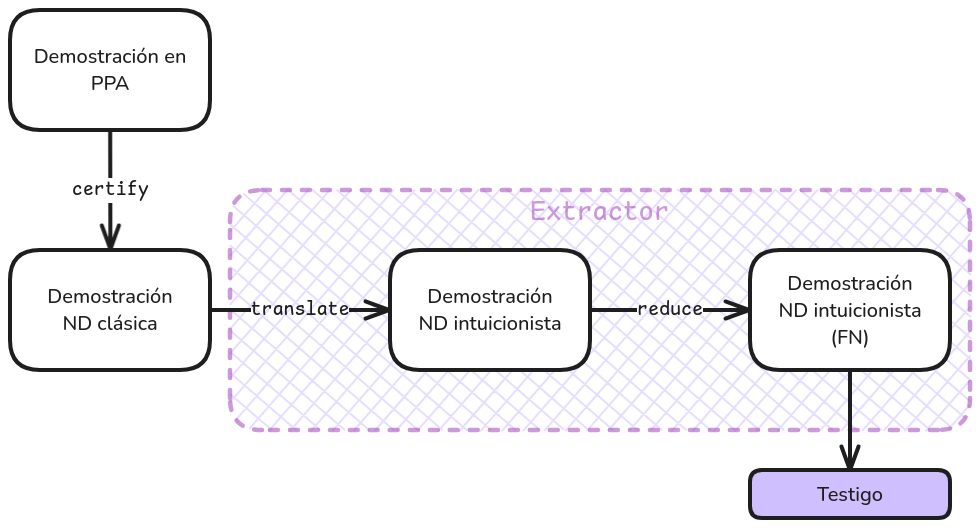
\includegraphics[scale=0.35]{img/fri-extract-strategy.png}
    \centering
    \caption{Estrategia de extracción de testigos}
    \label{fri:fig:strat}
\end{figure}

\section{Traducción de Friedman}

\subsection{Traducción de doble negación}

Existen muchos métodos que permiten embeber la lógica clásica en la
intuicionista. Un mecanismo general es la traducción de
\textbf{doble negación}, que tiene distintas variaciones. Una es la
\textit{Gödel-Gentzen} \cite{Avigad1998-FEFOFD}

\begin{definition}[Traducción \textit{Gödel-Gentzen}] Dada una fórmula $\form$
    se asocia con otra $\gN{\form}$. La traducción se define por inducción
    estructural.
    \begin{align*}
        \gN{\fFalse}                      & = \fFalse                                           \\
        \gN{\fTrue}                       & = \fTrue                                            \\
        \gN{\form}                        & = \fNot\fNot \form \quad \text{con $\form$ atómica} \\
        \gN{(\form \fAnd \formTwo)}       & = \gN{\form} \fAnd \gN{\formTwo}                    \\
        \gN{(\form \fOr \formTwo)}        & = \fNot(\fNot\gN{\form} \fAnd \fNot\gN{\formTwo})   \\
        \gN{(\form \fImp \formTwo)}       & = \gN{\form} \fImp \gN{\formTwo}                    \\
        \gN{(\forall \var . \form(\var))} & = \forall \var . \gN{\form(\var)}                   \\
        \gN{(\exists \var . \form(\var))} & = \fNot \forall \var . \fNot \gN{\form(\var)}
    \end{align*}
\end{definition}


\begin{definition}[Traducción de contextos]
    Se extiende a contextos de la forma esperable
    \[
        \gN{\ctx} = \{\gN{\form} \mid \form \in \ctx \}.
    \]
\end{definition}

\begin{notation*}
    Notamos,
    \begin{itemize}
        \item $\judgC$ para expresar que un juicio es derivable en lógica clásica,
              y $\judgI$ para intuicionista.
        \item $\someProof \proves \ctx \judG \form$ para expresar que $\someProof$ es una demostración de $\ctx \judG \form$. Equivalente a
              \AxiomC{$\someProof$}
              \noLine
              \UnaryInfC{$\ctx \judG \form$}
              \DisplayProof
    \end{itemize}
\end{notation*}

\begin{theorem}
    Si tenemos $\ctx \judgC \form$, luego $\gN{\ctx} \judgI \gN{\form}$.
\end{theorem}

Dada una demostración en lógica clásica, podemos obtener una en lógica
intuicionista de su traducción. Pero esto no es exactamente lo que queremos,
pues si quisiéramos extraer un testigo de una demostración de la fórmula
$\exists \var. \pred(\var)$, al traducirla nos quedaría
\(
\gN{(\exists \var. \pred(\var))}
= \fNot \forall \var . \fNot\fNot\fNot \pred(\var),
\)
que si bien su demostración sería intuicionista (y por lo tanto constructiva),
como no es de un $\exists$ al normalizarla no podremos hacer la extracción.

\subsection{El truco de Friedman}

La idea de Friedman \cite{miquel-friedman} es generalizar la traducción
Gödel-Gentzen reemplazando la negación intuicionista $\fNot \form \equiv A
    \rightarrow \bot$ por una relativa $\fNotR \form \equiv \form \rightarrow R$ que
está parametrizada por una fórmula arbitraria $R$. Esto nos va a permitir, con
una elección inteligente de $R$, traducir una demostración clásica de una
fórmula a una intuicionista, y usarla para demostrar \textbf{la fórmula
    original}. Esto nos permite reducirla y hacer la extracción. No va a ser posible para cualquier fórmula, sino las de una clase particular (de la forma
$\forall \varTwo_1 \dots \forall \varTwo_m . \exists \var_1 \dots \exists \var_k . \form$ o $\classPiTwo$)

\begin{definition}[Traducción de doble negación relativizada]
    \begin{align*}
        \transDNeg{\bot}                         & = \bot                                                             \\
        \transDNeg{\form}                        & = \fNotR\fNotR \form
        \quad \text{con $\form$ atómica}                                                                              \\
        \transDNeg{(\fNot \form)}                & = \fNot \transDNeg{\form}                                          \\
        \transDNeg{(\form \fAnd \formTwo)}       & = \transDNeg{\form} \fAnd \transDNeg{\formTwo}                     \\
        \transDNeg{(\form \fOr \formTwo)}        & = \fNotR(\fNotR\transDNeg{\form} \fAnd \fNotR\transDNeg{\formTwo}) \\
        \transDNeg{(\form \rightarrow \formTwo)} & = \transDNeg{\form} \rightarrow \transDNeg{\formTwo}               \\
        \transDNeg{(\forall x . \form)}          & = \forall x . \transDNeg{\form}                                    \\
        \transDNeg{(\exists x . \form)}          & = \fNotR \forall x . \fNotR \transDNeg{\form}
    \end{align*}
\end{definition}

\begin{theorem}
    \label{fri:thm:dneg-trans-classic-int}
    Si $\ctx \judgC \form$, luego $\transDNeg{\ctx} \judgI \transDNeg{\form}$
\end{theorem}
\begin{proof}
    Dada una demostración en deducción natural clásica $\ctx \judgC \form$, podemos traducirla recursivamente extendiendo la traducción de fórmulas a reglas de inferencia, así generando una demostración de $\transDNeg{\ctx} \judgI \transDNeg{\form}$.
    Este proceso está descrito en detalle en \fullref{fri:sec:proof-trans}
\end{proof}

Vamos a enunciar diferentes versiones de la traducción de Friedman en orden de sofisticación, según para qué clase de fórmulas funcionan. No solo ayuda a entenderla, sino que también fue el mismo enfoque con el que las implementamos. Cada una incluye a la anterior, por lo que en PPA solo quedó implementada la última.


\begin{definition}[Jerarquía aritmética de fórmulas]
    Clasifica las fórmulas en dos clases: $\classPi{n}$ y
    $\classSigma{n}$. Se define por inducción en $n$.

    \begin{itemize}
        \item Si $\anyForm$ es equivalente a una fórmula sin cuantificadores, está en
              $\classPi{0}$ y $\classSigma{0}$.
        \item Sean las clasificaciones $\classPi{n}$ y $\classSigma{n}$. Definimos para $n+1$.
              \begin{itemize}
                  \item Si $\anyForm$ es equivalente a una formula de la forma $\exists
                            \var_1 \dots \exists \var_k. \anyFormTwo$ donde $\anyFormTwo$ es
                        $\classPi{n}$, entonces $\anyForm$ es asignada la clasificación $\classSigma{n+1}$.

                  \item Si $\anyForm$ es equivalente a una formula de la forma $\forall
                            \var_1 \dots \forall \var_k. \anyFormTwo$ donde $\anyFormTwo$ es
                        $\classSigma{n}$, entonces $\anyForm$ es asignada la clasificación $\classPi{n+1}$.
              \end{itemize}
    \end{itemize}

    Una fórmula de $\classSigma{n}$ es equivalente a una que comienza con
    cuantificadores existenciales y alterna $n-1$ veces entre series de
    universales y existenciales. Mientras que una $\classPi{n}$ es análoga pero
    comenzando con universales.

    Las dos que más nos interesan son:
    \begin{itemize}
        \item $\classSigmaOne$: fórmulas de la pinta $\exists \var_1 \dots
                  \exists \var_k . \anyForm$.
        \item $\classPiTwo$: fórmulas de la pinta $\forall \varTwo_1 \dots \forall \varTwo_m . \exists \var_1 \dots \exists \var_k . \anyForm$
    \end{itemize}

    Una intuición detrás de los nombres de las clases puede ser
    \begin{itemize}
        \item $\Sigma$ es una sumatoria, que se puede interpretar como
              disyunciones (en el sentido del álgebra de Boole), y generalizar con un existencial.
        \item $\Pi$ análogamente pero con productoria, conjunciones y universales.
    \end{itemize}
\end{definition}

\subsection{Versiones de la traducción}

\begin{enumerate}
    \item \textbf{Fórmulas $\classSigmaOne$ atómicas} (\namedref{fri:thm:fri-sigmaone}):
          \[
              \exists \var . \form(\var) \text{ con } \form(\var) \text{ atómica.}
          \]
    \item \textbf{Fórmulas $\classPiTwo$ atómicas} (\namedref{fri:thm:fri-pitwo}):

          \[
              \forall \varTwo_1 \dots \forall \varTwo_n . \exists \var . \form(\var, \varTwo_1, \dots, \varTwo_n) \text{ con } \form(\dots) \text{ atómica}.
          \]

    \item \textbf{Fórmulas $\classPiTwo$ no atómicas} (\namedref{fri:thm:fri-pitwo-general}):

          \[
              \forall \varTwo_1 \dots \forall \varTwo_n . \exists \var . \anyForm(\var, \varTwo_1, \dots, \varTwo_n) \text{ con } \anyForm(\dots) \text{ no atómica}.
          \]

          Por ejemplo, podría ser $\pred(x) \fAnd \predTwo(\varTwo_1, \dots, \varTwo_n)$.
          Pero no podrá ser cualquier fórmula, por ej. no $\fNot(\pred(x) \fAnd \predTwo(\varTwo_1, \dots, \varTwo_n))$. En \todo{Cita} damos una caracterización.
\end{enumerate}

\begin{theorem}[Traducción de Friedman para fórmulas $\classSigmaOne$]
    \label{fri:thm:fri-sigmaone}

    Sea $\someProof$ una demostración clásica de $\exists \var . \form$, y
    $\form$ una fórmula atómica.
    Si tenemos
    \[
        \ctx \judgC \exists \var . \form,
    \]
    luego, podemos generar una demostración intuicionista de \textit{la misma fórmula}
    \[
        \transDNeg{\ctx} \judgI \exists \var . \form.
    \]
\end{theorem}
\begin{proof}

    Aplicando la traducción, tenemos que

    \begin{gather*}
        \transDNeg{\big(
            \someProof \proves \ctx \judgC \exists \var . \form
            \big)}\\
        \verteq\\
        \transDNeg{\someProof} \proves \transDNeg{\ctx} \judgI \fNotR \forall \var . \fNotR \fNotR \fNotR \form
    \end{gather*}

    luego, tomando $R = \exists \var . \form$ la fórmula que buscamos probar,

    \begin{align*}
        \transDNeg{\someProof} \proves & \transDNeg{\ctx} \judgI \fNotR \forall \var . \fNotR \fNotR \fNotR \form                                                                                                                  \\
        \iff                           & \transDNeg{\ctx} \judgI \fNotR \forall \var . \fNotR \form
                                       &                                                                                                                    & (\text{\namedref{fri:lemma:tnegr-elim}})                             \\
        =\                             & \transDNeg{\ctx} \judgI (\forall \var . (\form \rightarrow R)) \rightarrow R
                                       &                                                                                                                    & (\fNotR \form = \form \fImp R)                                       \\
        =\                             & \transDNeg{\ctx} \judgI (\forall \var . (\form \rightarrow \exists \var . \form)) \rightarrow \exists \var . \form &                                           & (R = \exists \var \form) \\
        \Rightarrow\                   & \transDNeg{\ctx} \judgI \exists \var . \form
                                       &                                                                                                                    & (\text{\namedref{fri:obs:forall-exists}})
    \end{align*}

    En deducción natural,

    \begin{prooftree}
        \def\defaultHypSeparation{\hskip .1in}
        \AxiomC{$\transDNeg{\someProof}$}
        \noLine
        \UnaryInfC{\(
            \transDNeg{\ctx} \judgI \fNotR \forall \var \fNotR \transDNeg{\form}
            \)}
        \AxiomC{}
        \RL{\ruleTNegRI}
        \admissibleRuleLine
        \UnaryInfC{$\transDNeg{\ctx}, \fNotR \form \judgI \fNotR \fNotR \fNotR \form$}
        \AxiomC{}
        \RL{\ruleAx}
        \UnaryInfC{$\transDNeg{\ctx}, \form \judgI \form$}
        \RL{\ruleExistsI}
        \UnaryInfC{$\transDNeg{\ctx}, \form \judgI R = \exists \var \form$}
        \RL{\ruleImpI}
        \UnaryInfC{$\transDNeg{\ctx} \judgI \fNotR \form$}
        \RL{\ruleCut}
        \admissibleRuleLine
        \BinaryInfC{$\transDNeg{\ctx} \judgI \fNotR \fNotR \fNotR \form$}
        \RL{\ruleForallI}
        \UnaryInfC{\(
            \transDNeg{\ctx} \judgI \forall \var \fNotR \transDNeg{\form}
            \)}
        \RL{\ruleImpE}
        \BinaryInfC{$\transDNeg{\ctx} \judgI \exists \var . \form$}
    \end{prooftree}
\end{proof}

\begin{obs}
    En la demostración del \namedref{fri:thm:fri-sigmaone} y las de esta sección, luego de la traducción de Friedman, todas las demostraciones deben ser intuicionistas para que sigan siendo constructivas.
\end{obs}

\begin{lemma}[Eliminación de triple negación relativa]\label{fri:lemma:tnegr-elim}
    $\fNotR\fNotR\fNotR \form \iff \fNotR \form$ y lo demostramos como dos reglas admisibles, una para cada lado

    \begin{multicols}{2}
        \begin{prooftree}
            \AxiomC{}
            \RL{\ruleTNegRE}
            \admissibleRuleLine
            \UnaryInfC{$\fNotR\fNotR\fNotR \form \judgI \fNotR \form$}
        \end{prooftree}

        \begin{prooftree}
            \AxiomC{}
            \RL{\ruleTNegRI}
            \admissibleRuleLine
            \UnaryInfC{$\fNotR \form \judgI \fNotR\fNotR\fNotR \form$}
        \end{prooftree}
    \end{multicols}
\end{lemma}
\begin{proof}

    Primero \ruleTNegRI{}

    \begin{prooftree}
        \AxiomC{}
        \RL{\ruleAx}
        \UnaryInfC{$\fNotR \form, \fNotR\fNotR \form \judgI \fNotR \fNotR \form$}
        \AxiomC{}
        \RL{\ruleAx}
        \UnaryInfC{$\fNotR \form, \fNotR\fNotR \form \judgI \fNotR \form$}
        \RL{\ruleImpE}
        \BinaryInfC{$\fNotR \form, \fNotR\fNotR \form \judgI R$}
        \RL{\ruleImpI}
        \UnaryInfC{$\fNotR \form \judgI \fNotR\fNotR\fNotR \form$}
    \end{prooftree}

    Ahora \ruleTNegRE{}

    \begin{prooftree}
        \AxiomC{}
        \RL{\ruleAx}
        \UnaryInfC{$\fNotR\fNotR\fNotR \form, \form \judgI \fNotR\fNotR\fNotR \form$}
        \AxiomC{}
        \RL{\ruleAx}
        \UnaryInfC{$\ctx \judgI \fNotR \form$}
        \AxiomC{}
        \RL{\ruleAx}
        \UnaryInfC{$\ctx \judgI \form$}
        \RL{\ruleImpE}
        \BinaryInfC{$\ctx = \fNotR\fNotR\fNotR \form, \form, \fNotR \form \judgI R$}
        \RL{\ruleImpI}
        \UnaryInfC{$\fNotR\fNotR\fNotR \form, \form \judgI \fNotR\fNotR \form$}
        \RL{\ruleImpE}
        \BinaryInfC{$\fNotR\fNotR\fNotR \form, \form \judgI R$}
        \RL{\ruleImpI}
        \UnaryInfC{$\fNotR\fNotR\fNotR \form \judgI \fNotR \form$}
    \end{prooftree}
\end{proof}

\begin{obs}\label{fri:obs:forall-exists}
    $\judgI \forall \var (\form \rightarrow \exists \var \form)$.
    Trivialmente, para cualquier $\var$ si vale $\form$ entonces va a existir un $\var$ tal que valga $\form$.
\end{obs}

\begin{theorem}[Traducción de Friedman para fórmulas $\classPiTwo$ atómicas]
    \label{fri:thm:fri-pitwo}

    Sea $\someProof$ una demostración clásica de
    \(
    \forall \varTwo_1 \dots \forall \varTwo_n .
    \exists \var .
    \form(\var, \varTwo_1, \dots, \varTwo_n)
    \)
    y $\form(\dots)$ una fórmula atómica

    Si tenemos
    \[
        \ctx \judgC
        \forall \varTwo_1 \dots \forall \varTwo_n .
        \exists \var .
        \form(\var, \varTwo_1, \dots, \varTwo_n),
    \]
    podemos generar una demostración intuicionista de la misma fórmula
    \[
        \transDNeg{\ctx} \judgI
        \forall \varTwo_1 \dots \forall \varTwo_n .
        \exists \var .
        \form(\var, \varTwo_1, \dots, \varTwo_n).
    \]
\end{theorem}
\begin{proof}
    Lo demostramos en deducción natural para un solo $\forall$. La demostración para una cantidad arbitraria es análoga y fácilmente generalizable a partir de esta. La estrategia consiste en primero introducir el $\forall$ reemplazando su variable por una fresca, para evitar conflictos con las variables usadas en la demostración original. Luego se procede a demostrar el $\exists$ de forma análoga al \namedref{fri:thm:fri-sigmaone}, usando la traducción de la demostración pero usando como $R$ no la fórmula original, sino el $\exists$ con la variable ligada por el $\forall$ reemplazada por la fresca.

    Tomando $R = \exists \var . \form(\var, \varTwo_0)$ y aplicando la traducción, tenemos que 

    \begin{gather*}
        \transDNeg{\big(
            \someProof \proves \ctx \judgC \forall \varTwo \exists \var . \form(\var, \varTwo)
            \big)}\\
        \verteq\\
        \transDNeg{\someProof} \proves
            \transDNeg{\ctx} \judgI
                \forall \varTwo \fNotR \forall \var . \fNotR \fNotR \fNotR \form(\var, \varTwo)
    \end{gather*}

    Luego

    \begin{prooftree}
        \AxiomC{$\tdn{\someProof}$}
        \noLine
        \UnaryInfC{$\tdn{\ctx} \judgI \forall \varTwo \fNotR \forall \var . \fNotR \tdn{\form(\var, \varTwo_0)}$}
        \RL{\ruleForallE}
        \UnaryInfC{$\tdn{\ctx} \judgI \fNotR \forall \var . \fNotR \tdn{\form(\var, \varTwo_0)}$}
        %
        \AxiomC{$\someProof_\forall$}
        \noLine
        \UnaryInfC{$\tdn{\ctx} \judgI\forall \var . \fNotR \tdn{\form(\var, \varTwo_0)}$}
        \RL{\ruleImpE}
        \BinaryInfC{$\tdn{\ctx} \judgI \exists \var . \form(\var, \varTwo_0)$}
        \RL{\ruleForallI}
        \UnaryInfC{$\tdn{\ctx} \judgI \forall \varTwo \exists \var . \form(\var, \varTwo)$}
    \end{prooftree}

    donde

    \begin{prooftree}
        \AxiomC{}
        \LL{\ruleTNegRI}
        \admissibleRuleLine
        \UnaryInfC{\(
            \tdn{\ctx}, \fNotR \form(\var, \varTwo_0) \judgI
                \fNotR \fNotR \fNotR \form(\var, \varTwo_0) 
        \)}
        \AxiomC{}
        \RL{\ruleAx}
        \UnaryInfC{\(
            \tdn{\ctx}, \form(\var, \varTwo_0) \judgI \form(\var, \varTwo_0)
        \)}
        \RL{\ruleExistsI}
        \UnaryInfC{\(
            \tdn{\ctx}, \form(\var, \varTwo_0) \judgI R = \exists \var . \form(\var, \varTwo_0)
        \)}
        \RL{\ruleImpI}
        \UnaryInfC{\(
            \tdn{\ctx} \judgI \fNotR \form(\var, \varTwo_0)
        \)}
        \RL{\ruleCut}
        \admissibleRuleLine
        \BinaryInfC{$\tdn{\ctx} \judgI \fNotR \fNotR \fNotR \form(\var, \varTwo_0)$}
        \RL{\ruleForallI}
        \LL{$\someProof_\forall =$}
        \UnaryInfC{$\tdn{\ctx} \judgI\forall \var . \fNotR \tdn{\form(\var, \varTwo_0)}$}
    \end{prooftree}
\end{proof}

\begin{corollary}[Instanciación de $\forall$]
    El \namedref{fri:thm:fri-pitwo} nos permite realizar la instanciación de las variables del $\forall$ eliminandolo e instanciando con el término que querramos. De esa forma, la demostración final es sobre un $\exists$, requerido para poder hacer la extracción sobre la demostración normalizada.
    Por ejemplo,
    \begin{prooftree}
        \AxiomC{(\ref{fri:thm:fri-pitwo})}
        \noLine
        \UnaryInfC{$\tdn{\ctx} \judgI \forall \varTwo \exists \var . \form(\var, \varTwo)$}
        \RL{\ruleForallE}
        \UnaryInfC{$\tdn{\ctx} \judgI \exists \var . \form(\var, \term)$}
    \end{prooftree}
\end{corollary}

\subsubsection{Formulas no atómicas}

Hasta ahora usamos la traducción de Friedman para traducir las demostraciones de una fórmula de clásica a intuicionista, manteniendo esa fórmula, siempre y cuando su sub-fórmula $\classSigma{0}$ sea \textbf{atómica}. Pero queremos generalizarlo a fórmulas como $\forall \varTwo \exists \var . \anyForm(\var, \varTwo)$ donde $\anyForm$ no sea atómica, por ejemplo $\form(\var) \fAnd \formTwo(\varTwo)$. Para ello, la única diferencia es en el uso de \ruleCut{}. Para fórmulas atómicas, tenemos

\begin{prooftree}
    \AxiomC{}
        \LL{\ruleTNegRI}
        \admissibleRuleLine
        \UnaryInfC{\(
            \tdn{\ctx}, \fNotR \form \judgI
                \fNotR \fNotR \fNotR \form 
        \)}
        \AxiomC{$\vdots$}
        \noLine
        \UnaryInfC{\(
            \tdn{\ctx} \judgI \fNotR \form
        \)}
        \RL{\ruleCut}
        \admissibleRuleLine
        \BinaryInfC{$\tdn{\ctx} \judgI \fNotR \tdn{\form} = \fNotR \fNotR \fNotR \tdn{\form}$}
\end{prooftree}

Que en donde aprovechamos que la traducción de fórmulas atómicas es $\fNotR \tdn{\form} = \fNotR \fNotR \fNotR \tdn{\form}$ y podemos llevarla a $\fNotR \form$ mediante la eliminación de la triple negación. Pero esto no es así para fórmulas que no sean atómicas. Para ello, enunciamos el \namedref{fri:lemma:notr-trans-intro}, el cual podemos usar para demostrar la traducción en el \namedref{fri:thm:fri-pitwo-general}.

\begin{lemma}[Congruencia de $\fNotR\fNotR$]
    \label{fri:lemma:dnegr-cong}
    Si $\form \judgI \form'$, luego $\fNot \fNot \form \judgI \fNot \fNot \form'$.
\end{lemma}

\begin{lemma}[Distributividad del $\fNotR$ sobre $\fAnd$]
    \label{fri:lemma:fnot-dist-over-and-right}
    \(
    \fNotR \form \fOr \fNotR \formTwo \judgI \fNotR(\form \fAnd \formTwo)
    \)
\end{lemma}

\begin{lemma}[Introducción de $\fNotR$]
    \label{fri:lemma:notr-trans-intro}
    Para algunas fórmulas $\form$, vale $\fNotR \form \judgI \fNotR \tdn{\form}$ y lo notamos con la regla admisible \ruleNotRTransI{}.
    
    No vale siempre, ya que en ese caso podríamos usar la traducción de Friedman para todas las fórmulas. Lo demostramos para las fórmulas descritas por la siguiente gramática (conjunciones y fórmulas atómicas)
    \[
        \form, \formTwo ::=
            \fFalse \mid \fTrue \mid \pred(\term_1, \dots, \term_n) 
            \mid \form \fAnd \formTwo
    \]
\end{lemma}
\begin{proof}
    La demostración se hace por inducción estructural en la fórmula.
    \begin{itemize}
        \item $\fFalse, \fTrue$ son triviales. Predicados con \ruleTNegRI{}.
        \item $\fNot, \fOr, \fImp, \exists, \forall$ no están demostradas. Debería ser posible para algunas, pero no es claro.
        \item $\fAnd$ es cierta para sub-fórmulas que cumplan con la hipótesis inductiva. Tiene algunos trucos.
    \end{itemize}

    Veamos esquemáticamente la demostración del $\fAnd$. En la \namedref{fri:fig:rIntro-and-dn} se puede ver el esquema en deducción natural.
    \begin{itemize}
        \item Debemos probar $\fNotR (\form \fAnd \formTwo) \judgI \fNotR \tdn{(\form \fAnd \formTwo)}$
        \item Intuitivamente, queremos llevarlo a $\fNotR (\form \fAnd \formTwo) \judgI \fNotR \tdn{\form} \fOr \fNotR \tdn{\formTwo}$. Pero esta demostración requiere el uso de \ruleDnegE{} para razonar por el absurdo, que no es cierto para lógica intuicionista (la demostración de esta equivalencia de De Morgan es clásica).
        \item Pero podemos usar un truco para razonar por el absurdo.
        \begin{itemize}
        \item Tenemos que $\fNotR \tdn{(\form \fAnd \formTwo)}$ es siempre equivalente a $\fNotR \fNotR (\fNotR \tdn{(\form \fAnd \formTwo)})$ por eliminación de triple negación.
        \item Podemos usar dos lemas auxiliares: $\fNotR \tdn{\form} \fOr \fNotR \tdn{\formTwo} \judgI \fNotR \tdn{(\form \fAnd \formTwo)}$ y la congruencia de la doble negación, que al ser doble es covariante: $\form \judgI \form' \Rightarrow \fNotR \fNotR \form \judgI \fNotR \fNotR \form'$ para demostrar 
        \[
            \fNotR \fNotR (\fNotR \tdn{\form} \fOr \fNotR \tdn{\formTwo})
            \judgI
            \fNotR \fNotR (\fNotR \tdn{(\form \fAnd \formTwo)})
        \]
        \end{itemize}
        \item Esto nos permite llevar $\fNotR (\form \fAnd \formTwo) \judgI \fNotR \tdn{(\form \fAnd \formTwo)}$ a \[\fNotR (\form \fAnd \formTwo) \judgI \fNotR \fNotR (\fNotR \tdn{\form} \fOr \fNotR \tdn{\formTwo})\]
        
        que se puede demostrar por el absurdo de forma análoga a la demostración clásica bien conocida.
    \end{itemize}

    \begin{sidewaysfigure}[ht]
        \begin{prooftree}
            \AxiomC{$\someProof_1$}
            \noLine
            \UnaryInfC{\(
                \fNotR (\form \fAnd \formTwo) \judgI
                \fNotR \fNotR \fNotR \tdn{(\form \fAnd \formTwo)}
            \)}
            \AxiomC{}
            \RL{\ruleTNegRE}
            \admissibleRuleLine
            \UnaryInfC{\(
                \fNotR \fNotR \fNotR \tdn{(\form \fAnd \formTwo)}
                \judgI \fNotR \tdn{(\form \fAnd \formTwo)}
            \)}
            \RL{\ruleCut}
            \BinaryInfC{\(
                \fNotR (\form \fAnd \formTwo) \judgI \fNotR \tdn{(\form \fAnd \formTwo)}
            \)}
        \end{prooftree}

        Donde,
        \begin{prooftree}
            \AxiomC{}
            \RL{(\namedref{fri:lemma:fnot-dist-over-and-right})}
            \UnaryInfC{\(
                \fNotR \tdn{\form} \fOr \fNotR \tdn{\formTwo}
                \judgI
                \fNotR \tdn{(\form \fAnd \formTwo)}
            \)}
            \RL{(\namedref{fri:lemma:dnegr-cong})}
            \UnaryInfC{\(
                \fNotR \fNotR (\fNotR \tdn{\form} \fOr \fNotR \tdn{\formTwo})
                \judgI
                \fNotR \fNotR \fNotR \tdn{(\form \fAnd \formTwo)}
            \)}
            \AxiomC{\textit{(demostración por el absurdo)}}
            \noLine
            \UnaryInfC{\(
                \fNotR (\form \fAnd \formTwo) \judgI
                \fNotR \fNotR (\fNotR \tdn{\form} \fOr \fNotR \tdn{\formTwo})
            \)}
            \RL{\ruleCut}
            \admissibleRuleLine
            \LL{$\someProof_1=$}
            \BinaryInfC{\(
                \fNotR (\form \fAnd \formTwo) \judgI
                \fNotR \fNotR \fNotR \tdn{(\form \fAnd \formTwo)}
            \)}
        \end{prooftree}
        \caption{Esquema de demostración de introducción de $\fNotR$ para el caso de $\fAnd$, ver \namedref{fri:lemma:notr-trans-intro}}.
        \label{fri:fig:rIntro-and-dn}
    \end{sidewaysfigure}
\end{proof}

\begin{theorem}[Traducción de Friedman para fórmulas $\classSigmaOne$ en general]
    \label{fri:thm:fri-pitwo-general}

    Sea $\someProof$ una demostración clásica de \(
    \forall \varTwo_1 \dots \forall \varTwo_n .
    \exists \var .
    \anyForm(\var, \varTwo_1, \dots, \varTwo_n)
    \), y
    $\anyForm(\var, \varTwo_1, \dots, \varTwo_n)$ una fórmula no atómica.
    Si tenemos
    \[
        \ctx \judgC
        \forall \varTwo_1 \dots \forall \varTwo_n .
        \exists \var .
        \anyForm(\var, \varTwo_1, \dots, \varTwo_n),
    \]
    podemos generar una demostración intuicionista de la misma fórmula
    \[
        \transDNeg{\ctx} \judgI
        \forall \varTwo_1 \dots \forall \varTwo_n .
        \exists \var .
        \anyForm(\var, \varTwo_1, \dots, \varTwo_n).
    \]
\end{theorem}
\begin{proof}
    Al igual que el \namedref{fri:thm:fri-pitwo} lo demostramos para un solo $\forall$. La demostración es análoga con la diferencia del uso del \namedref{fri:lemma:notr-trans-intro}: \ruleNotRTransI{}. En lugar de tener
    
\begin{prooftree}
    \AxiomC{}
        \LL{\ruleTNegRI}
        \admissibleRuleLine
        \UnaryInfC{\(
            \tdn{\ctx}, \fNotR \form \judgI
                \fNotR \fNotR \fNotR \form 
        \)}
        \AxiomC{$\vdots$}
        \noLine
        \UnaryInfC{\(
            \tdn{\ctx} \judgI \fNotR \form
        \)}
        \RL{\ruleCut}
        \admissibleRuleLine
        \BinaryInfC{$\tdn{\ctx} \judgI \fNotR \tdn{\form} = \fNotR \fNotR \fNotR \tdn{\form}$}
\end{prooftree}

    tenemos

    \begin{prooftree}
        \AxiomC{}
        \LL{\ruleNotRTransI}
        \admissibleRuleLine
        \UnaryInfC{\(
            \tdn{\ctx}, \fNotR \anyForm \judgI
                \fNotR \tdn{\anyForm}
        \)}
        \AxiomC{$\vdots$}
        \noLine
        \UnaryInfC{\(
            \tdn{\ctx} \judgI \fNotR \anyForm
        \)}
        \RL{\ruleCut}
        \admissibleRuleLine
        \BinaryInfC{$\tdn{\ctx} \judgI \fNotR \tdn{\anyForm}$}
    \end{prooftree}
\end{proof}

\subsection{Traducción de demostraciones}
\label{fri:sec:proof-trans}

Ya vimos como podemos usar la traducción de Friedman para, dada una traducción de la demostración, usarla para demostrar la misma fórmula. Pero aún no ahondamos en un detalle importante. En el \namedref{fri:thm:dneg-trans-classic-int} se introduce la necesidad de extender la traducción de doble negación relativizada de fórmulas a demostraciones, para poder traducir una demostración clásica a intuicionista. En esta sección lo vemos más en detalle.

La conversión se efectúa por inducción estructural en la demostración. Para cada regla de inferencia que demuestra $\form$, se genera una demostración a partir de ella para demostrar $\transDNeg{\form}$. La estrategia para hacerlo es similar para todas: usar la hipótesis inductiva para convertir las sub-demostraciones, y usarlas para generar la nueva demostración. Pero hay algunas que requieren un truco. Solo mostramos las interesantes.

\begin{itemize}
    \item \ruleAndI{} (\namedref{fri:lemma:trad-and-i}), \ruleAndEOne{}, \ruleAndETwo{}, \ruleImpI{}, \ruleImpE{},
          \ruleOrIOne{}, \ruleOrITwo{}, \ruleForallI{}, \ruleForallE{}, \ruleNotI{}, \ruleNotE{}, \ruleTrueI{}, \ruleAx{} son todas similares entre sí, por lo que solo mostramos una.
    \item \ruleExistsI{} (\namedref{fri:lemma:trad-exists-i}) es una regla simple pero más interesante que las anteriores, por la traducción de $\exists$.
    \item \ruleLEM{} (\namedref{fri:lemma:trad-lem}) es sumamente interesante, ya que se encuentra en el corazón de la traducción al ser la parte clave: ¿cómo traducimos el principio de razonamiento clásico que lo separa de la lógica intuicionista?
    \item \ruleFalseE{} (\namedref{fri:lemma:trad-false-e})  se prueba como lema por inducción estructural en la fórmula a demostrar.
    \item \ruleOrE{} (\namedref{fri:lemma:trad-or-e}) y \ruleExistsE{} son análogos y requieren un truco: usar la eliminación de la doble negación. Si bien al ser un principio de razonamiento clásico no vale para lógica intuicionista (por ser equivalente a LEM), lo que si vale es la eliminación de la doble negación relativizada: \ruleDnegRE{} (\namedref{fri:lemma:dnegr-e}).
\end{itemize}

\begin{lemma}[Traducción de \ruleAndI{}]
    \label{fri:lemma:trad-and-i}
    Dada una aparición de la regla \ruleAndI{},

    \begin{prooftree}
        \AxiomC{$\someProof_\form$}
        \noLine
        \UnaryInfC{$\ctx \judgI \form$}
        \AxiomC{$\someProof_\formTwo$}
        \noLine
        \UnaryInfC{$\ctx \judgI \formTwo$}
        \RL{\ruleAndI}
        \BinaryInfC{$\ctx \judgI \form \wedge \formTwo$}
    \end{prooftree}

    es posible traducirla generando una demostración de $\tdn{(\form \fAnd \formTwo)} = \tdn{\form} \fAnd \tdn{\formTwo}$.
\end{lemma}
\begin{proof}
    Por hipótesis inductiva, tenemos que
    \begin{itemize}
        \item \(
              \tdn{\someProof_\form} \proves
              \tdn{\ctx} \judgI
              \tdn{\form}
              \) y
        \item \(
              \tdn{\someProof_\formTwo} \proves
              \tdn{\ctx} \judgI
              \tdn{\formTwo}
              \)
    \end{itemize}

    Luego, podemos generar una demostración de $\tdn{\form} \fAnd \tdn{\formTwo}$

    \begin{prooftree}
        \AxiomC{$\tdn{\someProof_\form}$}
        \noLine
        \UnaryInfC{$\tdn{\ctx} \judgI \tdn{\form}$}
        \AxiomC{$\tdn{\someProof_\formTwo}$}
        \noLine
        \UnaryInfC{$\tdn{\ctx} \judgI \tdn{\formTwo}$}
        \RL{\ruleAndI}
        \BinaryInfC{$\tdn{\ctx} \judgI \tdn{\form} \fAnd \tdn{\formTwo}$}
    \end{prooftree}
\end{proof}

\begin{lemma}[Traducción de \ruleExistsI{}]
    \label{fri:lemma:trad-exists-i}
    Dada una aparición de la regla \ruleExistsI{},

    \begin{prooftree}
        \AxiomC{$\someProof$}
        \noLine
        \UnaryInfC{$\judg{\ctx}{\form\subst{\var}{\term}}$}
        \RL{\ruleExistsI}
        \UnaryInfC{$\judg{\ctx}{\exists \var. \form}$}
    \end{prooftree}

    es posible traducirla generando una demostración de $\tdn{\exists \var. \form} = \fNotR \forall \var . \fNotR \tdn{\form}$.
\end{lemma}
\begin{proof}
    Por hipótesis inductiva, tenemos que
    \(
        \tdn{\someProof} \proves
        \tdn{\ctx} \judgI
        \tdn{(\form \subst{\var}{\term})}
    \)

    Luego, podemos generar una demostración de $\fNotR \forall \var . \fNotR \tdn{\form}$

    \begin{prooftree}
        \AxiomC{}
        \RL{\ruleAx}
        \UnaryInfC{\(
            \ctx_1 \judgI \fNotR \forall \var \tdn{\form}
        \)}
        \RL{\ruleForallE}
        \UnaryInfC{\(
            \ctx_1 \judgI \fNotR \tdn{\form \subst{\var}{\term}}
        \)}
        \AxiomC{$\tdn{\someProof}$}
        \noLine
        \UnaryInfC{\(
            \ctx_1 \judgI \tdn{\form \subst{\var}{\term}}
        \)}
        \RL{\ruleImpE}
        \BinaryInfC{\(
            \ctx_1 = \tdn{\ctx}, \forall \var . \fNotR \tdn{\form} \judgI R
        \)}
        \RL{\ruleImpI}
        \UnaryInfC{\(
            \tdn{\ctx} \judgI \fNotR \forall \var . \fNotR \tdn{\form}
        \)}
    \end{prooftree}

\end{proof}

\begin{lemma}[Traducción de \ruleLEM{}]
    \label{fri:lemma:trad-lem}
    Dada una aparición de la regla \ruleLEM{},

    \begin{prooftree}
        \AxiomC{}
        \RL{\ruleLEM}
        \UnaryInfC{$\judg{\ctx}{\form \fOr \fNot \form}$}
    \end{prooftree}

    es posible traducirla generando una demostración de \[\tdn{\form \fOr \fNot \form} = \fNotR (\fNotR \tdn{\form} \fAnd \fNotR \fNotR \tdn{\form}).\]
\end{lemma}
\begin{proof}
    Como no hay HI, podemos demostrarlo para cualquier contexto $\ctx$.
    \begin{prooftree}
        \AxiomC{}
        \RL{\ruleAx}
        \UnaryInfC{\(
            \ctx_1
            \judgI \fNotR \tdn{\form} \fAnd \fNotR \fNotR \tdn{\form}
        \)}
        \RL{\ruleAndETwo}
        \UnaryInfC{\(
            \ctx_1
            \judgI \fNotR \fNotR \tdn{\form}
        \)}
        %
        \AxiomC{}
        \RL{\ruleAx}
        \UnaryInfC{\(
            \ctx_1
            \judgI \fNotR  \tdn{\form} \fAnd \fNotR \fNotR \tdn{\form}
        \)}
        \RL{\ruleAndEOne}
        \UnaryInfC{\(
            \ctx_1
            \judgI \fNotR \tdn{\form}
        \)}
        \RL{\ruleImpE}
        \BinaryInfC{\(
            \ctx_1 = \ctx,
            \fNotR \tdn{\form} \fAnd \fNotR \fNotR \tdn{\form}
            \judgI R
        \)}
        \RL{\ruleImpI}
        \UnaryInfC{\(
            \ctx \judgI
                \fNotR (\fNotR \tdn{\form} \fAnd \fNotR \fNotR \tdn{\form})
        \)}
    \end{prooftree}
\end{proof}
\begin{lemma}[Traducción de \ruleFalseE{}]
    \label{fri:lemma:trad-false-e}
    Dada una aparición de la regla \ruleFalseE{},

    \begin{prooftree}
        \AxiomC{$\someProof_\fFalse$}
        \noLine
        \UnaryInfC{$\judg{\ctx}{\fFalse}$}
        \RL{\ruleFalseE}
        \UnaryInfC{$\judg{\ctx}{\anyForm}$}    
    \end{prooftree}

    es posible generar una demostración de $\tdn{\anyForm}$ a partir de $\tdn{\fFalse} = R$.
\end{lemma}
\begin{proof}
    Por hipótesis inductiva (de inducción estructural sobre la demostración), tenemos que
    \begin{gather*}
        \tdn{\someProof_\fFalse} \proves \tdn{\ctx} \judgI \tdn{\fFalse}
        \\
        \verteq
        \\
        \someProof_R \proves \tdn{\ctx} \judgI R
    \end{gather*}
    Pero no es posible demostrar de forma directa $\tdn{\anyForm}$ a partir de $R$. Lo hacemos por inducción estructural en $\anyForm$. Todos los casos son parecidos. Por ejemplo, veamos un caso inductivo y uno base.
    
    \begin{itemize}
    \item Dada una conjunción $\form \fAnd \formTwo$, su traducción es $\tdn{\form} \fAnd \tdn{\formTwo}$. Por HI (de inducción estructural sobre la fórmula) a partir de $\someProof_R$ podemos probar $\tdn{\form}$ al igual que $\tdn{\formTwo}$. Luego,

    \begin{prooftree}
        \AxiomC{(HI)}
        \noLine
        \UnaryInfC{$\tdn{\ctx} \judgI \tdn{\formTwo}$}
        \AxiomC{(HI)}
        \noLine
        \UnaryInfC{$\tdn{\ctx} \judgI \tdn{\form}$}
        \RL{\ruleAndI}
        \BinaryInfC{$\tdn{\ctx} \judgI \tdn{\form} \fAnd \tdn{\formTwo}$}
    \end{prooftree}
    

    \item Dada una disyunción $\form \fOr \formTwo$, su traducción es $\fNotR (\fNotR \tdn{\form} \fAnd \fNotR \tdn{\formTwo})$. Luego, podemos demostrarlo sin usar la HI.
    
    \begin{prooftree}
        \AxiomC{$\someProof_R$}
        \noLine
        \UnaryInfC{\(
            \tdn{\ctx}, \fNotR \tdn{\form} \fAnd \fNotR \tdn{\formTwo} \judgI R
        \)}
        \RL{\ruleImpI}
        \UnaryInfC{\(
            \tdn{\ctx} \judgI \fNotR (\fNotR \tdn{\form} \fAnd \fNotR \tdn{\formTwo})
        \)}
    \end{prooftree}
    \end{itemize}

    El resto de los casos son análogos.
\end{proof}

\begin{lemma}[Eliminación de doble negación relativizada (\ruleDnegRE{})]
    \label{fri:lemma:dnegr-e}
    \todo{Enunciar y demostrar}
\end{lemma}

\begin{lemma}[Traducción de \ruleOrE{}]
    \label{fri:lemma:trad-or-e}
    \todo{Enunciar y demostrar}
\end{lemma}

\section{Normalización (o reducción)}

Repasemos en dónde estamos parados. Queremos extraer un testigo de la demostración de un existencial (i.e extraer de una demostración de  $\exists \var . \pred(\var)$ a un $\term$ tal que $\pred(\term)$). Partimos de una demostración escrita en el lenguaje de alto nivel PPA, que se certifica a una demostración en deducción natural \textit{clásica} (que tiene el problema para la reducción que no es constructiva). Mediante la traducción de Friedman, para cierto tipo de fórmulas ($\classPiTwo$), podemos convertir la demostración a \textit{intuicionista}. Ahora, queremos extraer el testigo a partir de ella. Eso lo podemos lograr \textbf{normalizando} la demostración. ¿De qué trata?

Intuitivamente, la estrategia que empleamos consiste en evitar \textit{desvíos superfluos} en una demostración, sucesivamente simplificándolos hasta que queda una demostración en forma normal. Por ejemplo, en la siguiente demostración se prueba $\form \fImp \form$ usando $(\form \fImp \form) \fAnd (\formTwo \fImp \formTwo)$ y demostrándo ambos por separado. Pero se puede demostrar de forma más directa, insertando directo la demostración de $\form \fImp \form$ y eliminado el desvío por el $\fAnd$.

\begin{figure}[H]
\[
    \AxiomC{}
    \RL{\ruleAx}
    \UnaryInfC{$\form \judG \form$}
    \RL{\ruleImpI}
    \UnaryInfC{$\judG \form \fImp \form$}
    \AxiomC{}
    \RL{\ruleAx}
    \UnaryInfC{$\formTwo \judG \formTwo$}
    \RL{\ruleImpI}
    \UnaryInfC{$\judG \formTwo \fImp \formTwo$}
    \RL{\ruleAndI}
    \BinaryInfC{$\judG (\form \fImp \form) \fAnd (\formTwo \fImp \formTwo)$}
    \RL{\ruleAndEOne{}}
    \UnaryInfC{$\judG \form \fImp \form$}
\DisplayProof
\quad
\rewrite
\quad
    \AxiomC{}
    \RL{\ruleAx}
    \UnaryInfC{$\form \judG \form$}
    \RL{\ruleImpI}
    \UnaryInfC{$\judG \form \fImp \form$}
    \DisplayProof
\]
\caption{Ejemplo de desvío y su normalización}
\end{figure}

Todos los desvíos que normalizamos se ven de esta forma: una \textbf{eliminación} seguida inmediatamente de su \textbf{introducción} correspondiente. Por ejemplo, \ruleAndEOne{} seguida de \ruleAndI{}.

Este proceso es análogo a las reducciones de cálculo $\lambda$. Más aún, existe
un isomorfismo entre demostraciones en deducción natural y términos de cálculo
$\lambda$: El isomorfismo Curry-Howard \cite{curry-howard-isomorphism}. Con él,
la normalización de demostraciones es el isomorfismo de las reducciones en
cálculo $\lambda$, su semántica. Por ejemplo, el isomorfismo nos permite pensar
en una conjunción como una tupla, y las eliminaciones como proyecciones. Luego,
podemos ver cómo la regla de normalización de la conjunción es isomorfa a la
regla de reducción de las proyecciones.

\begin{figure}[H]
    \begin{align*}
        \projectOne{\tuple{\lTerm_1}{\lTerm_2}} &\rewrite \lTerm_1\\
        \projectTwo{\tuple{\lTerm_1}{\lTerm_2}} &\rewrite \lTerm_2
    \end{align*}
    
    \[
        \reductionAnd
    \]
    \caption{Relación entre conjunciones y tuplas}
\end{figure}

De acá en adelante presentamos las reducciones directamente en deducción
natural, dado que es lo implementado en PPA. Usamos de forma intercambiable
\textit{reducción} y \textit{normalización}, pues en el fondo, son lo mismo.

\begin{obs}
    Es interesante notar que en las reducciones mencionadas en esta sección, no
    se explicita ni $\judgI$ ni $\judgC$ a diferencia de la traducción de
    Friedman. Esto es porque la normalización se puede ejecutar en ambos casos,
    con la diferencia de que si lo hacemos para una demostración de lógica
    clásica que use \ruleLEM{}, se traba cuando llega ahí y su forma normal no
    es muy útil.
\end{obs}

\subsection{Sustituciones}

No todas las reglas de reducción son igual de sencillas que $\fAnd$. Veamos el
caso de la implicación. Una eliminación seguida de una introducción tiene la siguiente forma.

\begin{prooftree}
    \AxiomC{$\someProof_\formTwo$}
    \noLine
    \UnaryInfC{$\ctx, \hypId: \form \judG \formTwo$}
    \RL{\ruleImpIh{\hypId}}
    \UnaryInfC{$\ctx \judG \form \fImp \formTwo$}
    \AxiomC{$\someProof_\form$}
    \noLine
    \UnaryInfC{$\ctx \judG \form$}
    \RL{\ruleImpE}
    \BinaryInfC{$\ctx \judG \formTwo$}
\end{prooftree}

Para eliminar el desvío, uno podría estar tentado a hacer directamente $\someProof_\formTwo \proves \ctx \judG \formTwo$ pero ¡\textbf{no sería correcto}! La demostración $\someProof_\formTwo$ requiere la hipótesis $\hypId : \form$. Lo correcto sería usar $\someProof_\formTwo$, pero reemplazando todas las ocurrencias de la hipótesis $\hypId$ por la demostración $\someProof_\form$. A continuación introducimos esa noción.

\begin{definition}[Hipótesis libres]
    Una hipótesis ocurre libre en una demostración si se cita sin ser definida. Las reglas que etiquetan y agregan hipótesis al contexto son las que las ligan (i.e. las mencionadas en \fullref{nd:sec:hyp-labels}: \ruleAxh{\hypId}, \ruleImpIh{\hypId}, \ruleNotIh{\hypId}, \ruleOrEh{\hypId}, \ruleExistsEh{\hypId})
\end{definition}

\begin{definition}[Hipótesis citadas por una demostración]
    Definimos el conjunto de hipótesis citadas por una demostración $\citedHyps{\someProof}$ como todas las hipótesis ligadas y libres que aparecen en ella.
\end{definition}

\begin{definition}[Sustitución de hipótesis]
    Notamos como \(\someProof \subst{\hypId}{\someProof'}\) a la sustitución sin capturas de todas las ocurrencias libres de una hipótesis $\hypId$ por una demostración $\someProofTwo$ en otra demostración $\someProof$. Una \textit{captura} ocurriría si en $\someProof$ se liga una hipótesis $\hypId_2 \neq \hypId$ tal que $\hypId_2 \in \citedHyps{\someProofTwo}$, se cite en $\someProofTwo$.
    
    Para evitar la captura, al igual que en la sustitución de variables, no podemos renombrar en $\someProofTwo$ (porque la hipótesis está ``libre''), sino que la reemplazamos por una hipótesis fresca en donde se liga la que genera el conflicto, en la sub-demostración de $\someProof$.
\end{definition}


Además, para la reducción del $\exists$ y $\forall$, necesitaremos extender la sustitución usual de variables (\namedref{nd:def:subst}) por términos a demostraciones. La implementación es análoga, evitando capturas y haciéndolo en una pasada de forma lineal.
\begin{definition}[Sustitución de variables en demostraciones]
    Notamos como $\someProof \subst{\var}{\term}$ a la sustitución sin capturas de todas las ocurrencias libres de una variable $\var$ por un término $\term$ en todas las partes de una demostración $\someProof$. Incluyendo los contextos.
    
    \duda{Hace falta definirlo más?}
\end{definition}


\duda{Pensamiento: Si no tuvieramos etiquetas, esta sustitución sería más fácil, no? Porque en lugar de reemplazar por ocurrencias de la etiqueta, reemplazas por veces que citas en un axioma una \textit{fórmula}, entonces si lo estás capturando te da igual, total es la misma fórmula. O se podrá romper?}

\subsection{Algoritmo de reducción}

\begin{figure}
    $$\reductionAnd$$
    \proofSpacing
    \[
        \reductionImp
    \]
    \duda{Por qué no directamente así?
        \AxiomC{$\someProof_\formTwo \subst{\hypId}{\someProof_\form}$}
        \noLine
        \UnaryInfC{$\ctx \judG \formTwo$}
        \DisplayProof
    }
    \proofSpacing
    \begin{gather*}
        \AxiomC{$\someProof_{\form_i}$}
    \noLine
    \UnaryInfC{$\ctx \judG \form_i$}
    \RL{\ruleOrI{i}}
    \UnaryInfC{$\ctx \judG \form_1 \fOr \form_2$}
    \AxiomC{$\someProof_{1}$}
    \noLine
    \UnaryInfC{$\ctx, \hypId_1 : \form_1 \judG \formTwo$}
    \AxiomC{$\someProof_{2}$}
    \noLine
    \UnaryInfC{$\ctx, \hypId_2 : \form_2 \judG \formTwo$}
    \RL{\ruleOrE{}}
    \TrinaryInfC{$\ctx \judG \formTwo$}
    \DisplayProof\\
    \rewrite \quad
    \left(
    \AxiomC{$\someProof_i$}
    \noLine
    \UnaryInfC{$\ctx, \hypId_i: \form_i \judG \formTwo$}
    \DisplayProof
    \right)\subst{\hypId_i}{\someProof_{\form_i}}
    \end{gather*}

    \[\reductionNot\]
    \proofSpacing
    \[
        \AxiomC{$\someProof$}
        \noLine
        \UnaryInfC{$\ctx \judG \form$}
        \RL{\ruleForallI}
        \UnaryInfC{$\ctx \judG \forall . \var \form$}
        \RL{\ruleForallE}
        \UnaryInfC{$\ctx \judG \form \subst{\var}{\term}$}
        \DisplayProof
        \rewrite \quad
        \left(
        \AxiomC{$\someProof$}
        \noLine
        \UnaryInfC{$\ctx \judG \form$}
        \DisplayProof
        \right)\subst{\var}{\term}
    \]
    \proofSpacing
    \[
        \AxiomC{$\someProof_\form$}
        \noLine
        \UnaryInfC{$\ctx \judG \form \subst{\var}{\term}$}
        \RL{\ruleExistsI}
        \UnaryInfC{$\ctx \judG \exists \var . \form$}
        \AxiomC{$\someProof_\formTwo$}
        \noLine
        \UnaryInfC{$\ctx, \hypId: \form \judG \formTwo$}
        \BinaryInfC{$\ctx \judG \formTwo$}
        \DisplayProof
        \rewrite \quad
        \left(
        \left(
            \AxiomC{$\someProof_\formTwo$}
            \noLine
            \UnaryInfC{$\ctx, \hypId: \form \judG \formTwo$}
            \DisplayProof
        \right)\subst{\var}{\term}
        \right)\subst{\hypId}{\someProof_\form}
    \]
    
    \caption{Reglas de reducción}
    \label{fri:fig:reduction-rules}
\end{figure}

A partir de todas las reglas de reducción (\namedref{fri:fig:reduction-rules}), dado que son \textit{pasos} que acercan la demostración sucesivamente a su versión normalizada, podemos implementarlo de forma análoga a DNF (\namedref{ppa:sec:dnf:algoritmo}) como la clausura reflexiva transitiva de la reducción de un paso (aplicarla 0 o más veces hasta que esté en forma normal). Al igual que DNF, también necesitaremos reglas de congruencia: si no hay una eliminación de una introducción para simplificar, se intentan de reducir recursivamente las sub-demostraciones.

En una primera implementación las sub-demostraciones las reducíamos en un paso, de izquierda a derecha. Por ejemplo, si teníamos una introducción de una conjunción, reducíamos de a un paso a la vez $\form \rewrite \form_1 \rewrite \form_2 \rewrite \dots \rewrite \form^{*}$ hasta llegar a $\form^{*}$ irreducible. Luego, lo mismo para $\formTwo$.

\proofTreeAndI

Pero esto resultó demasiado lento, dado que las demostraciones que reducimos son muy grandes (pues son generadas automáticamente), y si por ejemplo la sub-demostración que había que reducir estaba muy anidada, había que recorrerla toda para efectuar cada paso.

\begin{prooftree}
    \AxiomC{$\judg{\ctx}{\form}$}
    \AxiomC{$\judg{\ctx}{\formTwo}$}
    \RL{\ruleAndI}
    \BinaryInfC{$\judg{\ctx}{\form \wedge \formTwo}$}
    \UnaryInfC{$\vdots$}
    \noLine
    \UnaryInfC{$\someProof$}
\end{prooftree}

Además, las demostraciones eran de mayor profundidad por una mayor cantidad de iteraciones del algoritmo, lo que hacía que realizar sustituciones también sea costoso (pues hay que recorrer el árbol entero para ver las hipótesis citadas y realizar la sustitución).

Para solucionar este problema, implementamos una reducción en muchos pasos. En
la literatura se pueden encontrar muchas \textit{estrategias de reducción}
alternativas, que se clasifican en si reducen en un paso o muchos para cada
iteración de la clausura. Dentro de las de muchos, la que implementamos fue
\textbf{Gross-Knuth}, que reduce en muchos pasos todos los sub-términos posibles
al mismo tiempo. Aplicado a demostraciones, quiere decir que en un único paso de
reducción, al mismo tiempo reduciríamos $\form \fAnd \formTwo \rewrite \form^{*}
\fAnd \formTwo^{*}$. Esto hace que la convergencia sea mucho más rápida.

\duda{Probablemente falta rigurosidad en esta sección.}

\subsection{Limitaciones}

Implementamos una reducción sencilla, que solamente normaliza eliminaciones de introducciones de la misma regla. Pero hay otros patrones que dejamos afuera, 
para los cuales no llegamos a una forma normal. Entonces no siempre podremos extraer un testigo. Por ejemplo, en \fullref{fri:norm:fig:non-norm}, se puede observar una demostración sencilla que usa \lstinline{cases}. Pero al certificarla, traducirla y reducirla, no queda en una forma normal. Se repite dos veces \ruleExistsI{}, cuando se podría mover hacia la raíz del árbol y evitar repetirlo en cada rama del \ruleOrE{}. Esto hace que al intentar de extraer un testigo, el programa reporte una falla al no poder normalizar la demostración. Para soportar estos casos es necesario sofisticar la reducción, agregando otro tipo de reglas, que quedó fuera del alcance del trabajo.

\begin{figure}[H]
    \centering
    \begin{subfigure}[b]{0.4\textwidth}
        \caption{Programa de PPA}
        \lstinputlisting{listings/extract/or-fail.ppa}
    \end{subfigure}
    \par\bigskip
    \begin{subfigure}[b]{1\textwidth}
        \caption{Demostración traducida y reducida}
        \begin{prooftree}
            \AxiomC{}
            \RL{\ruleAx}
            \UnaryInfC{$\ctx \judgI p(k) \fOr q(k)$}
            %
            \AxiomC{$\someProof_L$}
            \noLine
            \UnaryInfC{$\ctx, p(k) \judgI \exists y . r(y)$}
            %
            \AxiomC{$\someProof_R$}
            \noLine
            \UnaryInfC{$\ctx, q(k) \judgI \exists y . r(y)$}
            \RL{\ruleOrE}
            \TrinaryInfC{$\ctx \judgI \exists y . r(y)$}
        \end{prooftree}

        con $\someProof_L$ definido de la siguiente forma, y $\someProof_R$ simétrico.

        \begin{prooftree}
            \AxiomC{}
            \RL{\ruleAx}
            \UnaryInfC{$\ctx, p(k) \judgI p(k) \fImp r(k)$}
            \AxiomC{}
            \RL{\ruleAx}
            \UnaryInfC{$\ctx, p(k) \judgI p(k)$}
            \BinaryInfC{$\ctx, p(k) \judgI r(k)$}
            \RL{\ruleExistsI}
            \LL{$\someProof_L =$}
            \UnaryInfC{$\ctx, p(k) \judgI \exists y . r(y)$}
        \end{prooftree}
    \end{subfigure}
    \par\bigskip
    \begin{subfigure}[b]{1\textwidth}
        \caption{Demostración en forma normal}
        \begin{prooftree}
            \AxiomC{}
            \RL{\ruleAx}
            \UnaryInfC{$\ctx \judgI p(k) \fOr q(k)$}
            %
            \AxiomC{$\someProof_L$}
            \noLine
            \UnaryInfC{$\ctx, p(k) \judgI r(y)$}
            %
            \AxiomC{$\someProof_R$}
            \noLine
            \UnaryInfC{$\ctx, q(k) \judgI r(k)$}
            \RL{\ruleOrE}
            \TrinaryInfC{$\ctx \judgI r(k)$}
            \RL{\ruleExistsI}
            \UnaryInfC{$\ctx \judgI \exists y . r(y)$}
        \end{prooftree}

        con $\someProof_L$ y $\someProof_R$ análogas al caso anterior, pero sin
        \ruleExistsI{}.
    \end{subfigure}
    \caption{Ejemplo de demostración no normalizada}
    \label{fri:norm:fig:non-norm}
\end{figure}

\section{Manteniendo el contexto}

Problema con normalización: axiomas, hay que traducirlos para que la traducción de Friedman funcione. Solución? Dejar los axiomas originales y demostrar su traducción. No funciona siempre.

\begin{lemma}[Introducción de la traducción $\fNot\fNot$]
    Se reduce a transintro
\end{lemma}

\todo{Enunciar y demostrar}

\section{Otros métodos de extracción}

\todo{Hablar sobre y citar classical realizability, no tengo ni idea.}

Buena intro acá https://www.degruyter.com/document/doi/10.1515/9783110324921.11/html?lang=en

In the past years, many computational interpretations of Classical Arithmetic havebeen put forward.  Under a first classification, they fall into two large categories:directandindirectinterpretations.   Among  the  indirect  interpretations  one  findsthe  negative  translations  followed  either  by  Dialectica  interpretations  [13],  [30](see e.g.   Kohlenbach [19]) or by intuitionistic realizability interpretations com-bined with Friedman’s translation [13] (see e.g. Berger and Schwichtenberg [10]).Among the direct interpretations, there are different versions of Classical Realiz-ability (Krivine’s [22] and Avigad’s [6]), there is Coquand game semantics [11],